\chapter{Loading a text}
\label{chap-text}

One of the main functionalities of Unitex is to search a text for expressions.
To do that, texts have to undergo a set of preprocessing steps that  normalize
non-ambiguous forms and split the text  in sentences. Once these operations are
performed, the electronic dictionaries are applied to the texts. Then one  can
search more effectively in the texts by using  grammars.

\bigskip
\noindent This chapter describes the different steps for text preprocessing.


\section{Selecting a language}
\index{Selecting a language}\index{Language selection}
When starting Unitex, the program asks you to choose the language in which you
want to work (see figure~\ref{fig-language-selection}). The languages
displayed are the ones that are present in the \verb+Unitex+ system directory and those that
are  installed in your personal working directory. If you use a language for the
first time, Unitex copies the system directory for this language to your personal
directory, except for the dictionaries in order to save disk space.

\bigskip
\noindent WARNING: If
you already have a personal directory for a given language, Unitex won't try to
copy system data into it. So, if an update has modified a resource file other
than a dictionary, you will have to copy by yourself this file, or to delete your
personal directory for this language, and let Unitex rebuild it properly.

\bigskip
\noindent 
Choosing the language allows Unitex to find certain files, for example the
alphabet file. \index{File!alphabet} You can change the language at any time by
choosing "Change Language..." in the "Text" menu. If you change the language, the
program will close all windows related to the current text, if there are any. The
active language is indicated in the title bar of the graphical interface.

\begin{figure}[!h]
\begin{center}
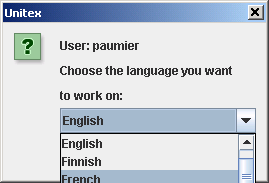
\includegraphics[width=6.2cm]{resources/img/fig2-1.png}
\caption{\label{fig-language-selection}Language selection when starting
Unitex}
\end{center}
\end{figure}


\section{Text formats}
\label{section-conversion-texte-unicode}
\index{Text!formats}
\index{Corpus|see{Text}}
\index{Unicode}
Unitex works with Unicode texts. Unicode is a standard that describes a universal
character code. Each character is given a unique number, which allows for
representing texts without having to take into account  the proprietary codes on
different machines and/or operating systems. Unitex uses a two-byte
representation of the Unicode 3.0 standard, called Unicode Little-Endian (for
more details, see \cite{UNICODE}).

\bigskip
\index{File!transcoding}
\noindent Texts that come with Unitex are already in Unicode format. If you try
to open a text that is not in Unicode, the program proposes to convert it
(see figure~\ref{auto-transcoding}).
This conversion is based on the current language: if you are working in French,
Unitex proposes to convert your text\,\footnote{Unitex also proposes to
automatically convert graphs and dictionaries that are not in Unicode
Little-Endian.} assuming that it is coded using a French code page. By default,
Unitex proposes to either replace the original text or to rename the original
file by inserting \verb$.old$ at the beginning of  its extension. For example, if
one has an ASCII file named \verb$biniou.txt$, the conversion process will create
a copy of this ASCII file named \verb$biniou.old.txt$, and will replace the
contents of \verb$biniou.txt$ with its equivalent in Unicode.


\begin{figure}[!h]
\begin{center}
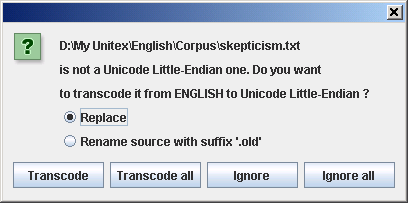
\includegraphics[width=10cm]{resources/img/fig2-2.png}
\caption{\label{auto-transcoding}Automatic conversion of a non-Unicode text}
\end{center}
\end{figure}

\noindent If the encoding suggested by default is not correct  or if you want to
rename the file differently than with the suffix \verb$.old$, you must use the "More options..." 
button. This allows you to choose source and
target encodings of the documents to be converted (see figure~\ref{transcoding}). By default,
the selected source encoding is that which corresponds to the current language
and the destination encoding is Unicode Little-Endian. You can modify these choices by selecting
any source and target encodings. Thus, if you wish, you can convert your data
into other encodings, as for example UTF-8 in order for instance to create web pages. The button
"Add Files" enables you to select the files to be converted. The button "Remove Files" makes it
possible to remove a list of files erroneously selected. The button "Transcode" will start the
conversion of all the selected files. If an error occurs with a file is
processed (for example, a file which is already in Unicode), the 
conversion continues with the next file.


\begin{figure}[!h]
\begin{center}
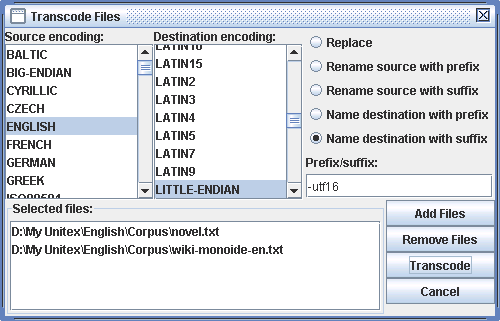
\includegraphics[width=12cm]{resources/img/fig2-3.png}
\caption{\label{transcoding}Transcoding files}
\end{center}
\end{figure}

\noindent To obtain a text in the right format, you can also use a text
processor like the free software from OpenOffice.org  (\cite{OpenOffice}) or Microsoft Word, and
save your document with the format "Unicode text".
In OpenOffice Writer, you have to choose the "Coded Text (*.txt)" format and then
select the "Unicode" encoding in the configuration window as shown on figure
\ref{OfficeWriter}.

\begin{figure}[!h]
\begin{center}
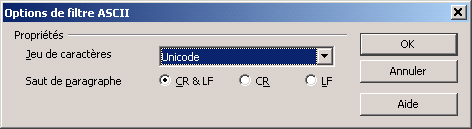
\includegraphics[width=12.5cm]{resources/img/fig2-4.png}
\caption{\label{OfficeWriter}Saving in Unicode with OpenOffice Writer}
\end{center}
\end{figure}

\noindent By default, the encoding proposed on a PC is always Unicode
Little-Endian. The texts thus obtained do not contain any formatting information anymore (fonts,
colors , etc.) and are ready to be used with Unitex.

\bigskip
\noindent 
You can change the default encoding to UTF16LE, UTF16BE or UTF8 in the 'Encoding' tab via the Preference  command in the Info menu. This encoding is valid for the current language only.

\begin{figure}[!h]
\begin{center}
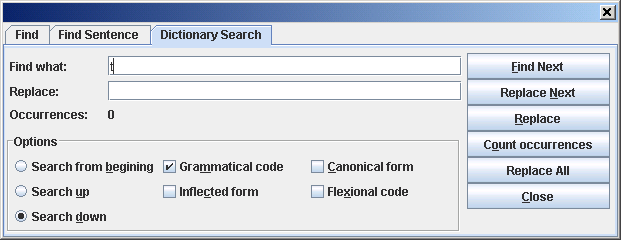
\includegraphics[width=10cm]{resources/img/fig2-5.png}
\caption{\label{OfficeWriter}Setting the default encoding for current language}
\end{center}
\end{figure}

\section{Editing text files}
For small texts, you also have the possibility of using the text editor integrated into Unitex,
accessible via the "Open..." command in the "File Edition" menu".
\index{Integrated text editor} This editor offers search and replace
functionalities  for the texts and dictionaries handled by Unitex. To use it,
click on the "Find" icon. You will then see a window  divided into three parts.
The "Find" part corresponds to the usual search operations. If you open a text
split into sentences, you can base your search on sentence numbers 
in the "Find Sentence" part. Lastly, the "Search Dictionary" part,
visible in figure~\ref{dictionary-search}, enables you to carry out operations
concerning the electronic dictionaries. In particular, you can   search by
specifying if it concerns  inflected forms, lemmas, grammatical and semantic
and/or inflectional codes. Thus, if you want to search for all the verbs which
have the  semantic feature \verb$t$, which indicates
transitivity, you just have to search for  \verb$t$ by clicking on "Grammatical
code". You will get the matching entries without confusion  with all the other
occurrences of the letter \verb$t$.


\begin{figure}[!h]
\begin{center}
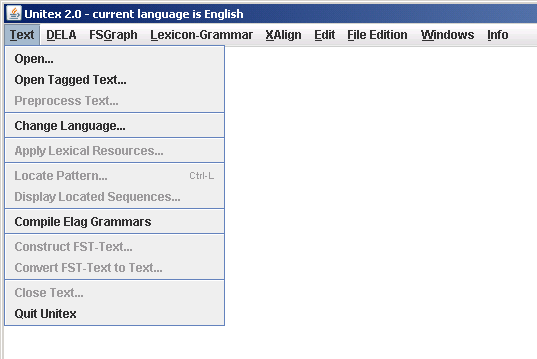
\includegraphics[width=15cm]{resources/img/fig2-6.png}
\caption{Searching an electronic dictionary for the semantic feature \texttt{t}\label{dictionary-search}}
\end{center}
\end{figure}


\section{Opening a text}
%Unitex deals with two types of text files. \index{File!text}
%The files with the extension \verb+.snt+ are text files preprocessed by Unitex
%which are ready to be manipulated by the different system functions. The files
%ending with \verb+.txt+ are raw files.
%To use a text, open the \verb+.txt+ file by clicking on "Open..." in the "Text"
%menu. Choose the file type "Raw Unicode Texts" and select your text.

Unitex deals with several types of documents. \index{File!text}
The files with the extension \verb+.snt+ are text files preprocessed by Unitex 
which are ready to be manipulated by the different system functions. 
You can also load raw files ending with \verb+.txt+, or XML and HTML files. 
To open any of these files, click on "Open..." in the
"Text" menu. You can there choose the file type ("Raw Unicode Texts", "XML files", "HTML files", "Unitex Texts").
If you open XML or HTML files, foo.xml for example, it will be preprocessed in order to remove non textual content. This will produce a foo.xml.txt file containing only the textual content of the original file. The resulting \verb+.txt+ file will be processed to produce a \verb+.snt+ file


\begin{figure}[!h]
\begin{center}
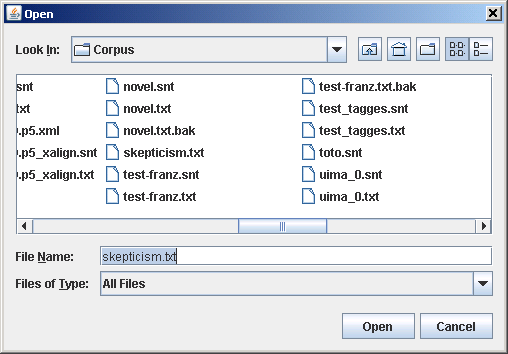
\includegraphics[width=14cm]{resources/img/fig2-7.png}
\caption{Text Menu}
\end{center}
\end{figure}

\begin{figure}[!h]
\begin{center}
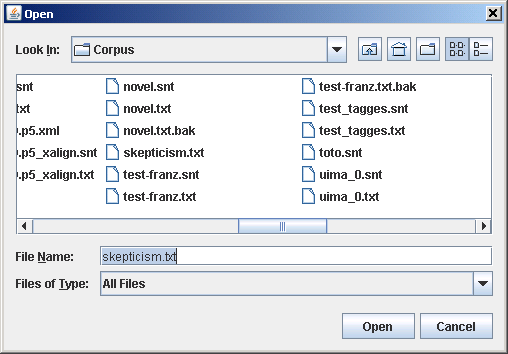
\includegraphics[width=13cm]{resources/img/fig2-8.png}
\caption{Opening a Unicode text}
\end{center}
\end{figure}

 

\section{Preprocessing a text}
\index{Text!preprocessing}
After a text is selected, Unitex offers to preprocess it. Text preprocessing
consists of performing the following operations: normalization of separators,
splitting into sentences, normalization of non-ambiguous forms, tokenization and 
application of dictionaries. If you choose not to preprocess the text, it 
will nevertheless be normalized and tokenized, since
these operations are necessary for all further Unitex operations. It is always
possible to carry out the preprocessing later by clicking on "Preprocess Text..."
in the "Text" menu. 

\begin{figure}[!h]
\begin{center}
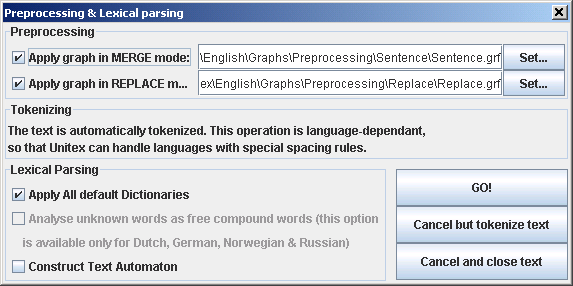
\includegraphics[width=15cm]{resources/img/fig2-9.png}
\caption{Preprocessing Window\label{fig-preprocessing-frame}}
\end{center}
\end{figure}

\bigskip
\noindent 
If you choose to preprocess the text, Unitex proposes to parameterize it
as in the window shown in figure~\ref{fig-preprocessing-frame}.
The option "Apply FST2 in MERGE mode" is used to split the text into sentences.
The option "Apply FST2 in REPLACE mode" is used to make replacements in the text,
especially for the normalization of non-ambiguous forms. With the option "Apply
All default Dictionaries" you can apply dictionaries in the DELA format
(Dictionnaires Electroniques du LADL).\index{DELA} The option "Analyze unknown
words as free compound words" is used in Norwegian for correctly analyzing
compound words  constructed via concatenation of simple forms.  Finally, the
option "Construct Text Automaton" is used to build the text automaton. This
option is deactivated by default, because it consumes a large amount of memory
and disk space if the text is too large. The construction of the text automaton
is described in chapter~\ref{chap-text-automaton}.

\bigskip
\noindent NOTE: If you click on "Cancel but tokenize text", the program will
carry out the normalization of separators and split the text into tokens. Click
on "Cancel and close text" to cancel the operation.

\subsection{Normalization of separators}
\index{Normalization!of separators}\index{Separators!word}\index{Word separators}\index{Text!normalization}
The standard separators are the space, the tab and the newline characters. There
can be several separators following each other, but since this isn't useful for
linguistic analyses, separators are normalized according to the following rules:

\begin{itemize}
  \item a sequence of separators that contains at least one newline is replaced by a single newline
  
  \item all other sequences of separators are replaced by a single space.
\end{itemize}

\bigskip
\noindent 
The distinction between space and newline is maintained at this point because the
presence of newlines may have an effect on the process of splitting the text into
sentences. The result of the normalization of a text named  \verb+my_text.txt+ is
a file in the same directory as the \verb+.txt+ file and is named
\verb+my_text.snt+. \index{File!\verb+.snt+}

\bigskip
\noindent NOTE: When the text is preprocessed using the graphical interface, a
directory named

% do not remove this line jump 
\noindent \verb+my_text_snt+ is created immediately after normalization.
This directory, called text directory,  \index{Directory!text}
\index{Text!directory} contains all the data associated with this text.



\subsection{Splitting into sentences}
\label{section-sentence-splitting}
\index{Splitting!into sentences}\index{Text!splitting into sentences}
\index{Grammars!splitting into sentences}
Splitting texts into sentences is an important preprocessing step since  this
helps in determining the units for linguistic processing. The splitting is used
by the text automaton construction program. In contrast to what one might think,
detecting sentence boundaries is not a trivial problem. Consider the following
text:

\bigskip
\textit{The family has urgently called Dr. Martin.}

\bigskip \noindent The full stop that follows \textit{Dr} is followed by a word
beginning with a capital letter. Thus it may be considered as the end of the
sentence, which would be wrong. To avoid the kind of problems caused by the
ambiguous use of punctuation, grammars are used to  describe the different
contexts for the end of a sentence.
Figure~\ref{fig-example-sentence-splitting} shows an example grammar for
sentence splitting (for French sentences).

\bigskip
\noindent When a path of the grammar recognizes a sequence in the text and when
this path produces the sentence delimiter symbol \verb+{S}+
\index{\verb+{S}+}\index{Sentence delimiter}, this symbol is inserted into the
text.

\bigskip
\noindent The path shown at the top of
figure~\ref{fig-example-sentence-splitting} recognizes the sequence consisting
of a question mark and a word beginning with a capital letter and inserts the 
symbol \verb+{S}+ between the question mark and
the following word. The following text:

\bigskip
\textit{What time is it? Eight o' clock.}

\bigskip
\noindent will be converted to:

\bigskip
\textit{What time is it ?\{S\} Eight o' clock.}

\bigskip
\noindent A  grammar for end-of-sentence detection may use the following
special symbols, or meta-symbols:

\index{\verb+<E>+}\index{Epsilon|see{<E>}}
\index{\verb+<MOT>+}\index{\verb+<MIN>+}\index{\verb+<MAJ>+}\index{\verb+<PRE>+}\index{\verb+<NB>+}
\index{\verb+<PNC>+}\index{\verb+<^>+}\index{\verb+#+}\index{Meta-symbols}
\index{\verb+<WORD>+}\index{\verb+<UPPER>+}\index{\verb+<LOWER>+}\index{\verb+<FIRST>+}
\begin{itemize}
  \item <E> : empty word, or epsilon. Recognizes the empty sequence;
  \item <WORD> : recognizes any sequence of letters (<MOT> is deprecated);
  \item <LOWER> : recognizes any sequence of letters in lower case (<MIN> is deprecated);
  \item <UPPER> : recognizes any sequence of letters in upper case (<MAJ> is deprecated);
  \item <FIRST> : recognizes any sequence of letters that begins with an upper case letter (<PRE> is deprecated);
  \item <NB> : recognizes any sequence of digits (1234 is recognized but not 1
  234); \item <PNC> : recognizes the punctuation symbols \verb+ ; , ! ? :+ and the
  inverted exclamation points and question marks in Spanish and some Asian
  punctuation letters; \item <\verb+^+> : recognizes a newline; \item \verb+#+ :
  prohibits the presence of a space.
\end{itemize}

\begin{figure}[!h]
\begin{center}
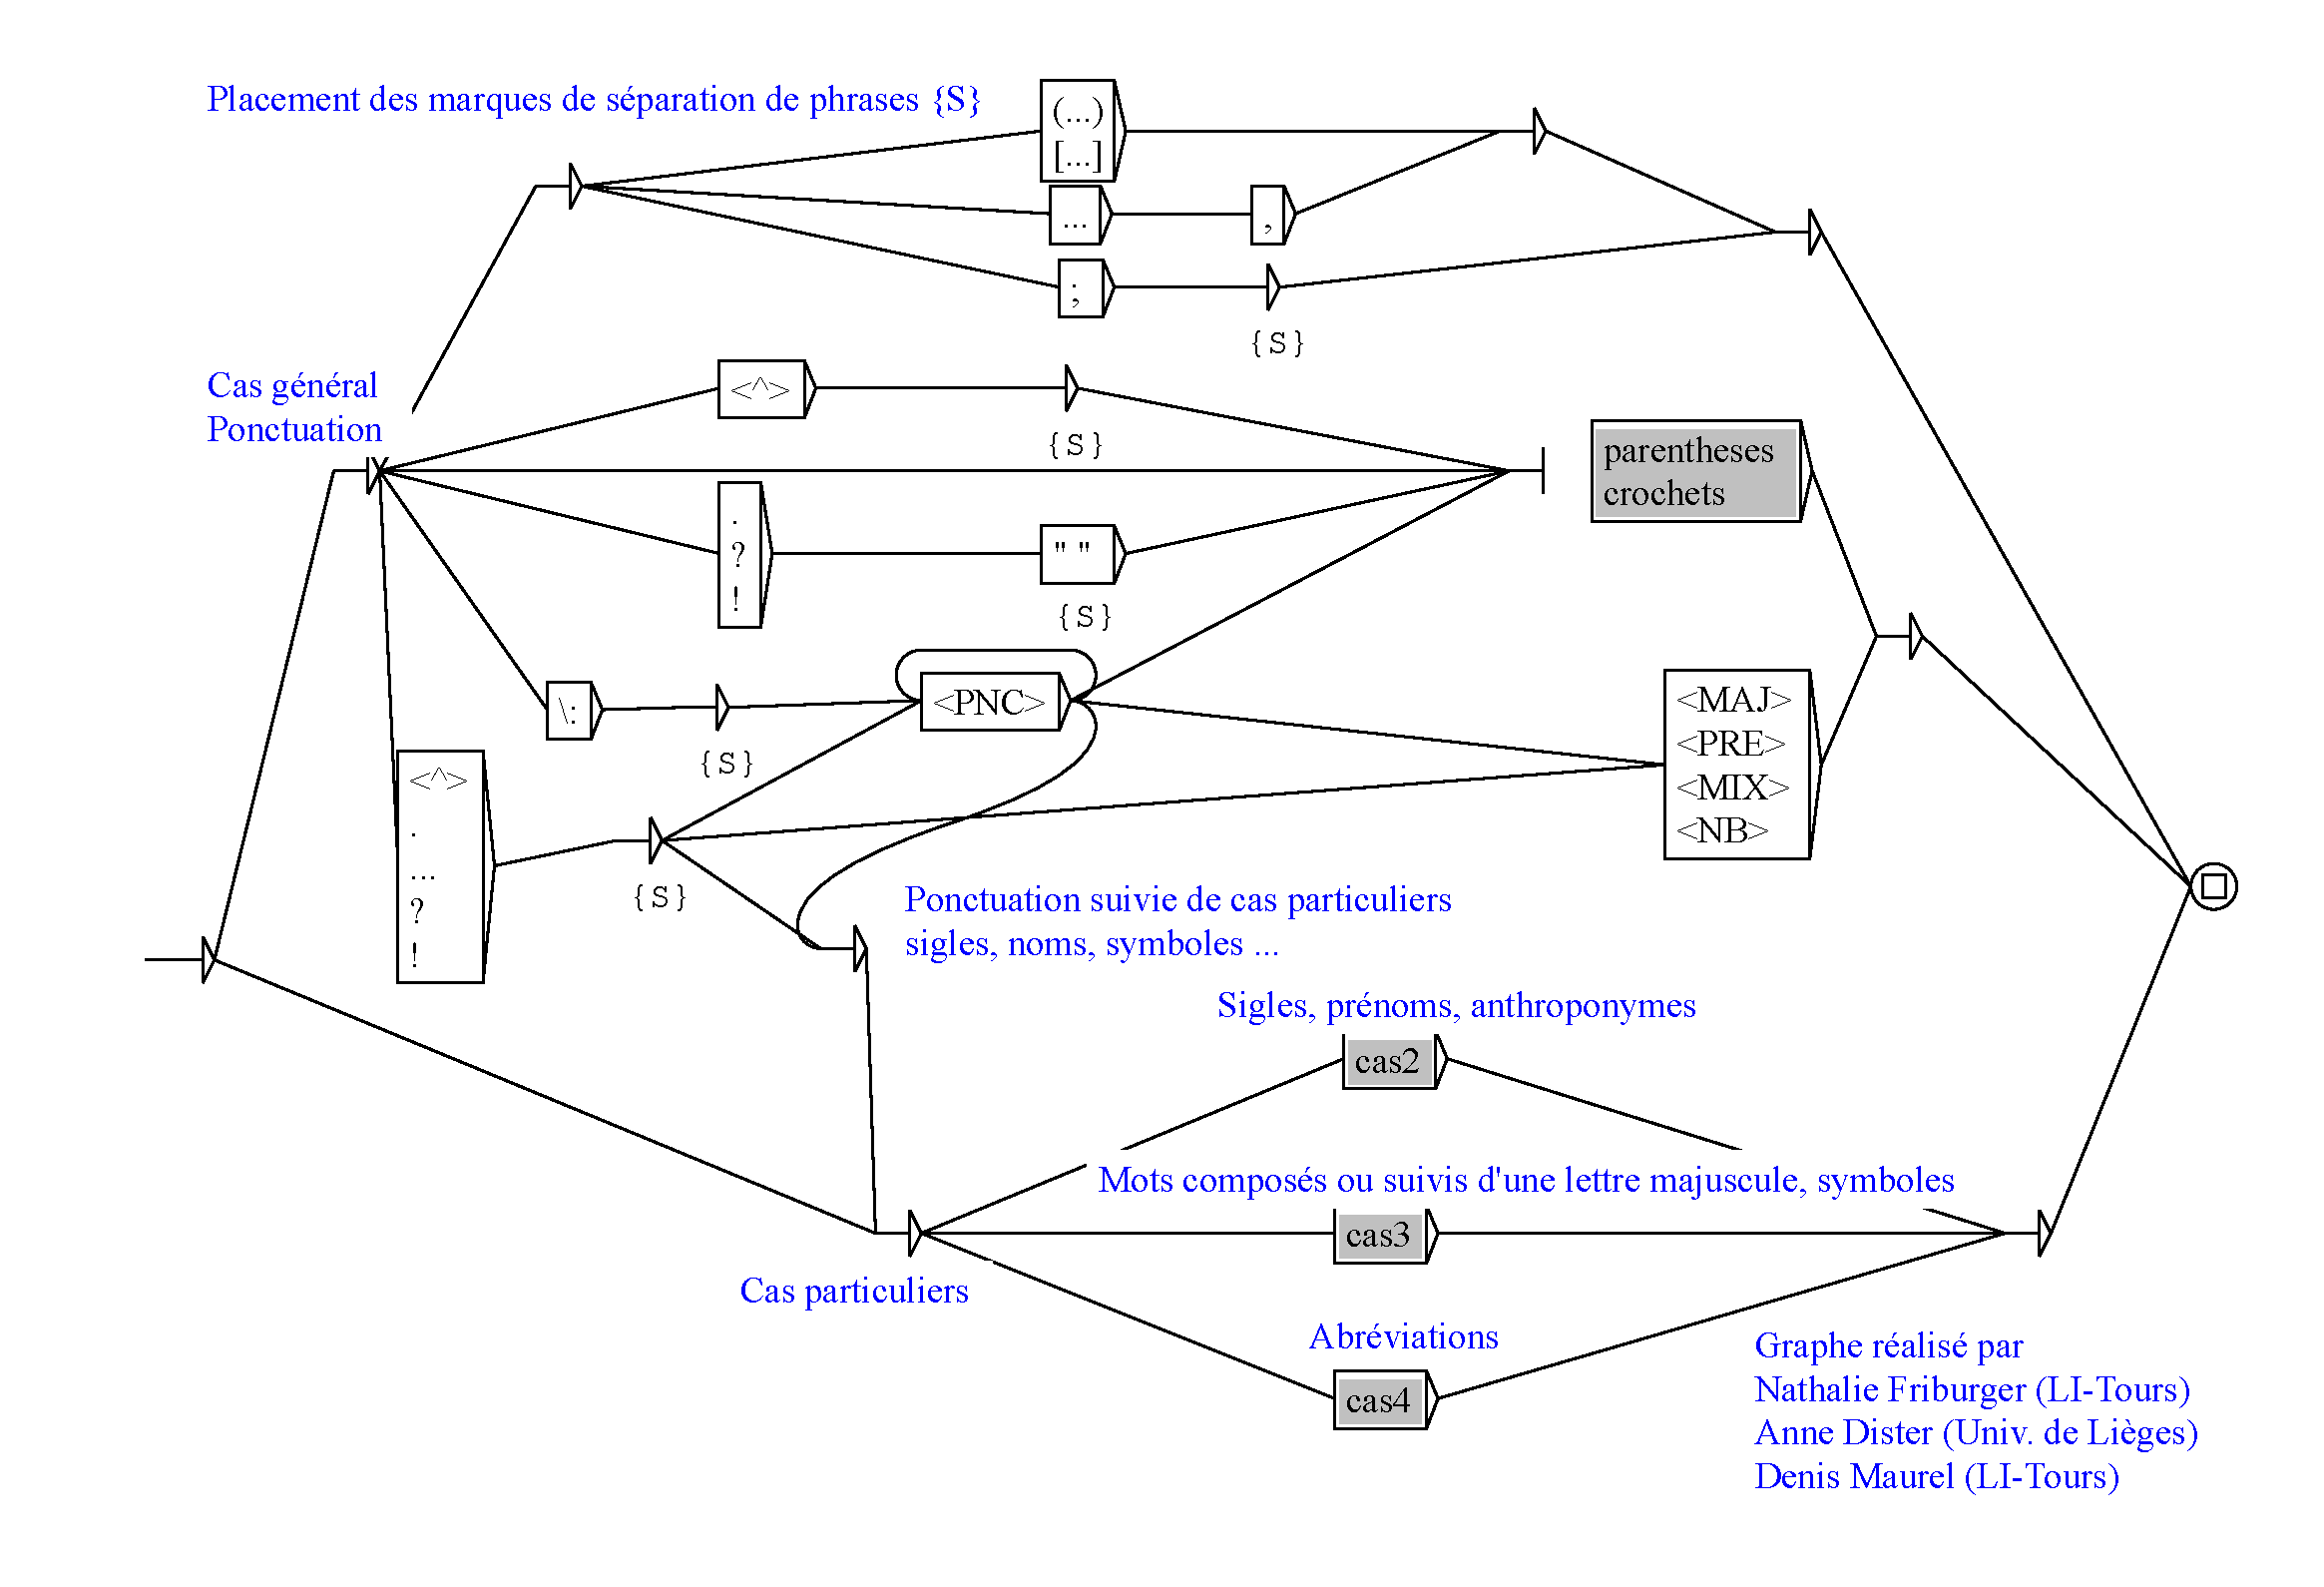
\includegraphics[width=15cm]{resources/img/fig2-10.pdf}
\caption{Sentence splitting grammar for
French\label{fig-example-sentence-splitting}}
\end{center}
\end{figure}

\bigskip
\noindent By default, the space is optional between two boxes. If you want to prohibit the
presence of the space you have to use the special character  \verb+#+. At the
opposite, if you want to force the presence of the space, you must use the
sequence \verb+" "+. Lower and upper case letters are defined by an alphabet
file\index{File!alphabet} (see chapter~\ref{chap-file-formats}). For
more details on grammars, see chapter~\ref{chap-grammars}.\index{Alphabet}
For more information about sentence boundary detection, see
\cite{ameliorer-decoupage-en-phrases}. The grammar used here is named
\verb+Sentence.fst2+ and can be found in the following directory:
\index{File!\verb+Sentence.fst2+}

\bigskip
\verb+/(user home directory)/(language)/Graphs/Preprocessing/Sentence+

\bigskip
\noindent This grammar is applied to a text with the \verb+Fst2Txt+ program
\index{\verb+Fst2Txt+}\index{External programs!\verb+Fst2Txt+} in
MERGE mode.\index{MERGE} This has the effect that the output produced
by the grammar, in this case the symbol \verb+{S}+, is inserted into
the text. This program takes a \verb+.snt+ file and modifies it.


\subsection{Normalization of non-ambiguous forms}
\index{Normalization!of non-ambiguous forms}
\index{Grammars!normalization!of non-ambiguous forms}

Certain forms present in texts can be normalized (for example, the English
sequence "\textit{I'm}" is equivalent to "\textit{I am}"). You may want to
replace these forms according to your own needs. However, you have to be careful
that the  forms normalized  are unambiguous or that the removal of ambiguity has
no undesirable consequences.

\bigskip
\noindent For instance, if you want to normalize "\textit{O'clock}" to "\textit{on the
clock}", it would be a bad idea to replace "\textit{O'}" by "\textit{on the }",
because a sentence like:

\bigskip
\textit{John O'Connor said: "it's 8 O'clock"}

\bigskip
\noindent would be replaced by the following incorrect sentence:

\bigskip
\textit{John on the Connor said: "it's 8 on the clock"}

\bigskip
\noindent Thus, one needs to be very careful when using the
normalization grammar. One needs to pay attention to spaces as well. 
For example, if one replaces "'re" by "are", the sentence:

\bigskip
\textit{You're stronger than him.}

\bigskip
\noindent will be replaced by:

\bigskip
\textit{Youare stronger than him.}

\bigskip
\noindent To avoid this problem, one should explicitly insert a space,
\textit{i.e.} replace "\textit{'re}" by "\textit{ are}".

\bigskip
\noindent The accepted symbols for the normalization grammar are the same as the ones
allowed for the sentence splitting grammar. The normalization grammar is called
\verb+Replace.fst2+ and can be found in the following directory:

\bigskip \verb+/(home directory)/(active language)/Graphs/Preprocessing/Replace+

\bigskip
\noindent As in the case of sentence splitting, this grammar is applied using the
\verb+Fst2Txt+ \index{External programs!\verb+Fst2Txt+}\index{\verb+Fst2Txt+}
program, but in REPLACE mode, which means that input sequences recognized by the
grammar are replaced by the output sequences that are produced.
Figure~\ref{fig-normalization-grammar} shows a grammar that
normalizes verbal contractions in English.

\begin{figure}[!p]
\begin{center}
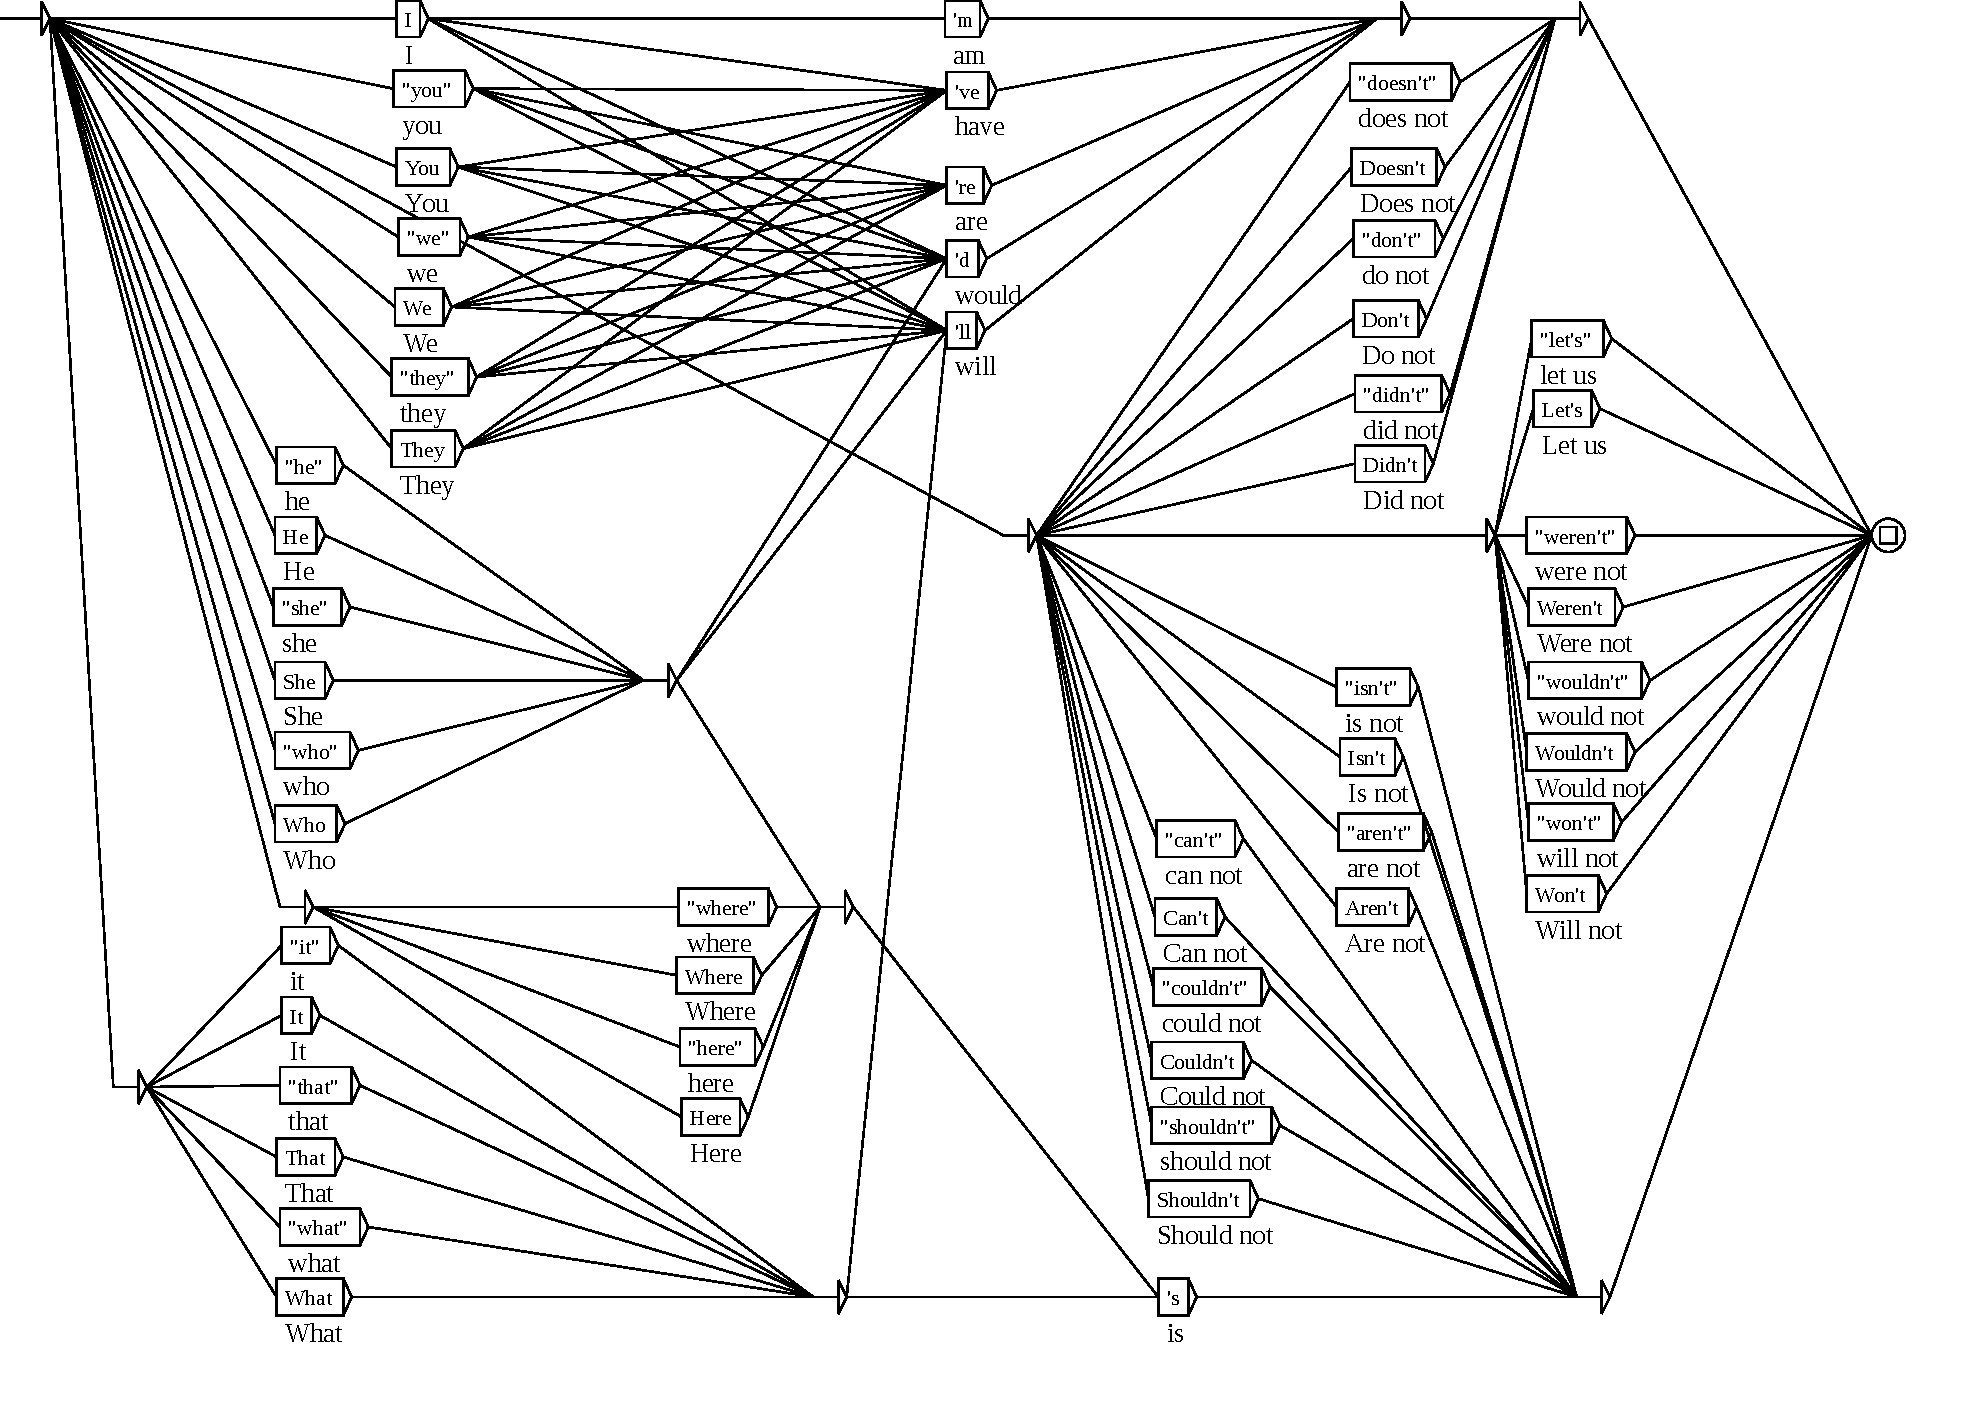
\includegraphics[height=17cm,angle=90]{resources/img/fig2-11.pdf}
\caption{Normalization of English verbal
contractions\label{fig-normalization-grammar}}
\end{center}
\end{figure}



\subsection{Splitting a text into tokens}
\index{Text!tokenization}
\index{Text!splitting into tokens}
\index{Splitting!into tokens}
\index{Token}
\index{Tokenization}
\label{tokenization}
Some languages, in particular Asian languages, use separators that are different
from the ones used in  western languages. Spaces can be forbidden, optional, or
mandatory. In order to better cope with these particularities,  Unitex splits
texts in a language dependent way. Thus, languages like English are treated as
follows:

\bigskip
\noindent A token can be:
\begin{itemize}
  \item the sentence delimiter \verb+{S}+; \item the stop marker
  \verb+{STOP}+.\index{\verb${STOP}$} This token is a special one that can
  NEVER be matched in any way by a grammar. It can be used to bound elements
  in a corpus. For instance, if a corpus is made of news separated by
  \verb+{STOP}+, it will be impossible that a grammar matches a sequence that
  overlaps the end of a news and the beginning of the following news;
  \item a lexical tag \verb+{aujourd'hui,.ADV}+; \item a contiguous sequence of
  letters (the letters are defined in the language alphabet file);
  \index{File!alphabet}
  \item one (and only one) non-letter character, i.e. all characters not defined
  in the alphabet file of the current language; if it is a newline, it is replaced by
  a space.
\end{itemize}

\bigskip
\noindent For other languages, tokenization is done on a character by character
basis, except for the sentence delimiter \verb+{S}+, the \verb+{STOP}+ marker
and lexical tags. This simple tokenization is fundamental for the use of Unitex,
but limits the optimization of search operations for patterns.

\bigskip
\noindent Regardless of the tokenization mode, newlines in a text are
replaced by spaces. Tokenization is done by the \verb+Tokenize+\index{\verb+Tokenize+}
\index{External programs!\verb+Tokenize+} program. This program creates several
files that are saved in the text directory:
\begin{itemize}
  \item \verb+tokens.txt+ contains the list of tokens in the order in which they are found in the text;
  \index{File!\verb+tokens.txt+}
  \item \verb+text.cod+ contains an integer array; every
  integer corresponds to the index of a token in the file \verb+tokens.txt+;
  \index{File!\verb+text.cod+}
  \item \verb+tok_by_freq.txt+ contains the list of tokens sorted by frequency;
  \index{File!\verb+tok_by_freq.txt+}
  \item \verb+tok_by_alph.txt+ contains the list of tokens in alphabetical order;
  \index{File!\verb+tok_by_alph.txt+}
  \item \verb+stats.n+ contains some statistics about the text. \index{File!\verb+stats.n+}
\end{itemize}

\bigskip
\noindent Tokenizing the text:

\bigskip
\textit{A cat is a cat.}

\bigskip
\noindent returns the following list of tokens: \textit{A} SPACE \textit{cat is a .}

\bigskip
\noindent You will observe that tokenization is case sensitive (\textit{A} and
\textit{a} are two distinct tokens), and that each token is listed only once.
Numbering these tokens from 0 to 5, the text can be represented by a sequence of
numbers (integers) as described in the following table:

\bigskip
\begin{table}[h]
\begin{center}
\begin{tabular}{|p{2.8cm}||c|c|c|c|c|c|c|c|c|c|c|c|}
\hline
Token number               & 0 & 1 & 2 & 1 & 3 & 1 & 4 & 1 & 2 & 5
\\
\hline
Corresponding token & \textit{A} &   & \textit{cat} &   & \textit{is} &  & \textit{a}
& & \textit{cat} & \textit{.}
\\
\hline
\end{tabular}
\caption{Representation of the text \textit{A cat is a cat.}}
\end{center}
\end{table}

\bigskip
\noindent For more details, see chapter~\ref{chap-file-formats}.

\begin{figure}[!h]
\begin{center}
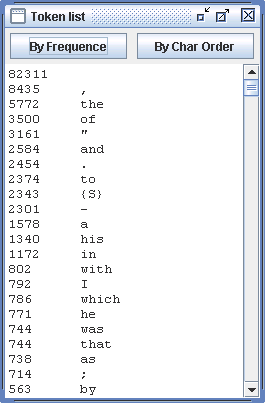
\includegraphics[height=10cm]{resources/img/fig2-12.png}
\caption{Tokens of an English text sorted by frequency}
\end{center}
\end{figure}



\subsection{Applying dictionaries}
\label{text-applying-dictionaries}
\index{Dictionaries!applying}
\index{Lexical!resources|see {Dictionaries}}
Applying dictionaries consists of building the subset of dictionaries  consisting
only of forms that are present in the text. Thus, the result of applying a
English dictionary to the text \textit{Igor's father in law is ill} produces a
dictionary of the following simple words:\index{Words!simple}

\bigskip
\begin{verbatim}
father,.N+Hum:s
father,.V:W:P1s:P2s:P1p:P2p:P3p
ill,.A
ill,.ADV
ill,.N:s
in,.A
in,.N:s
in,.PART
in,.PREP
is,be.V:P3s
is,i.N:p
law,.N:s
law,.V:W:P1s:P2s:P1p:P2p:P3p
s,.N:s
\end{verbatim}

\bigskip
\noindent as well as a dictionary of compound words consisting of a single
entry:\index{Words!compound}

\bigskip
\begin{verbatim}
father in law,.N+NPN+Hum+z1:s
\end{verbatim}

\bigskip
\noindent Since the sequence \textit{Igor} is neither a simple English word nor a part of a
compound word, it is treated as an unknown word. \index{Words!unknown} The
application of dictionaries is done through the program \verb+Dico+.
\index{\verb+Dico+}\index{External programs!\verb+Dico+} The three files produced
(\verb+dlf+ for simple words, \verb+dlc+ for compound words and \verb+err+ for
unknown words) are placed in the text directory. The \verb+dlf+ and \verb+dlc+
files are called text dictionaries.  \index{Dictionaries!text}
\index{File!\verb+dlf+}
\index{File!\verb+dlc+}\index{File!\verb+err+}

\bigskip
\noindent As soon as the dictionary look-up  is finished, Unitex displays the sorted lists
of simple, compound and unknown words found in a new window.
Figure~\ref{fig-Dico-application-results} shows the result for an
English text.

\begin{figure}[!ht]
\begin{center}
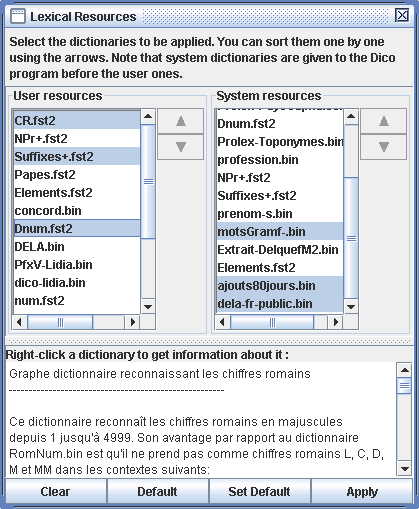
\includegraphics[width=12cm]{resources/img/fig2-13.png}
\caption{Result after applying dictionaries to an English text\label{fig-Dico-application-results}}
\end{center}
\end{figure}

\bigskip
\noindent It is also possible to apply dictionaries without preprocessing the text. In
order to do this, click on "Apply Lexical Resources..." in the "Text" menu.
Unitex then opens a window (see
figure~\ref{fig-Dico-configuration}) in which you can select
the list of dictionaries to apply.

\begin{figure}[!ht]
\begin{center}
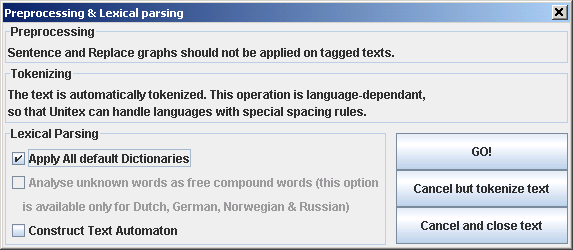
\includegraphics[width=10cm]{resources/img/fig2-14.png}
\caption{Parameterizing the application of dictionaries\label{fig-Dico-configuration}}
\end{center}
\end{figure}

\bigskip
\noindent The list "User resources" lists all dictionaries present in the
directory

% DO NOT REMOVE THIS LINE JUMP!
\noindent \verb+(current language)/Dela+ of the user. The dictionaries installed
in the system are listed in the scroll list  named "System resources". Use the
<Ctrl+click> combination to select several dictionaries. System dictionaries
will be applied prior to user dictionaries. Within the system or user list, you
can fix the order of dictionaries using the up and down arrows, as shown on
figure \ref{fig-Dico-configuration}. The button "Set
Default" allows you to define the current selection of dictionaries  as the
default. This default selection will then be used during preprocessing if you
activate the option "Apply All default Dictionaries".\index{Dictionaries!default
selection} If you right-click on a dictionary name, the associated documentation,
if any, will be displayed in the lower frame of the window.


\subsection{Analysis of compound words in Dutch, German, Norwegian and Russian}
\index{Norwegian!free compound words}\index{German!free compound words}\index{Dutch!free compound words}
\index{Russian!free compound words}
\index{Analysis of free compound words!in Germanic languages}\index{Words!compound!in Germanic languages}
\index{Analysis of free compound words!in Russian}\index{Words!compound!in Russian}
\label{section-Norwegian-compound-words}
In certain languages like Norwegian, German and others, it is possible to form
new compound words by concatenating  together other words. For example, the word
\textit{aftenblad} meaning \textit{evening journal} is obtained by combining the
words \textit{aften} (\textit{evening}) et \textit{blad} (\textit{journal}). The
\verb+PolyLex+ program \index{\verb+PolyLex+}\index{External
programs!\verb+PolyLex+} parses the list of unknown words after the application
of dictionaries and tries to analyze each of these words as a compound word. If
a word has at least one analysis as a compound word,  it is removed from the
list of unknown words and the lines produced for this word are appended to the
simple word text dictionary.



\section{Opening a tagged text}
A tagged text is a text containing words with lexical tags enclosed in braces:

\bigskip
\textit{I do not like the \{square bracket,.N\} sign! \{S\}}

\bigskip
\noindent Such tags can be used to avoid ambiguities. In the previous example,
it will be impossible to match \textit{square bracket} as the combination of two
simple words.

\bigskip
\noindent However, the presence of these tags can alter the application of
preprocessing graphs. To avoid complications, you can use the "Open Tagged
Text..." command in the "Text" menu. With it, you can open a tagged text and skip
the application of preprocessing graphs, as shown on Figure
\ref{preprocess-tagged-text}.

\bigskip
\begin{figure}[!h]
\begin{center}
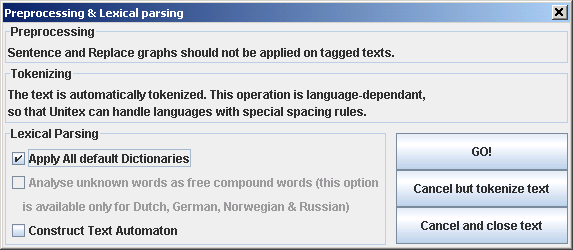
\includegraphics[width=14cm]{resources/img/fig2-15.png}
\caption{Preprocessing a tagged text\label{preprocess-tagged-text}}
\end{center}
\end{figure}
